\subsection{Simulation of the Neutron Background with GEANT4}
\label{secNRalphaN_GEANT4}

The neutron energy spectra calculated with SOURCES-4A and the calculated total production rates have been used as input for Monte Carlo simulations to predict the neutron-induced nuclear recoil background in the XENON100 experiment. 

\begin{figure}[!b]
\centering
\subfigure[]{
%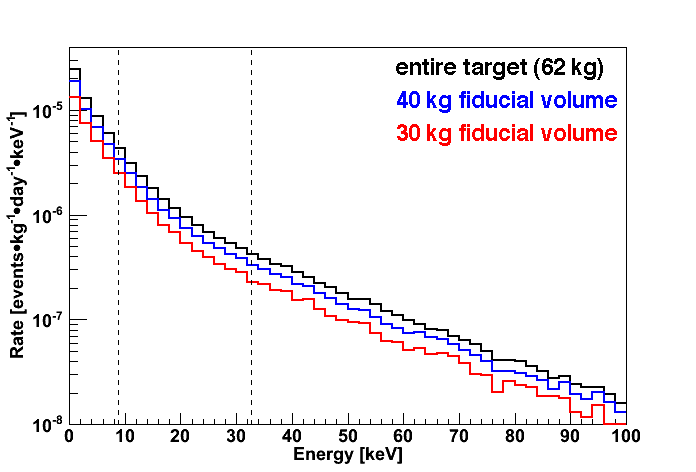
\includegraphics[width=0.475\linewidth]{plots/NRalphaN/nrBG_FV_NRelastics_mod.png}
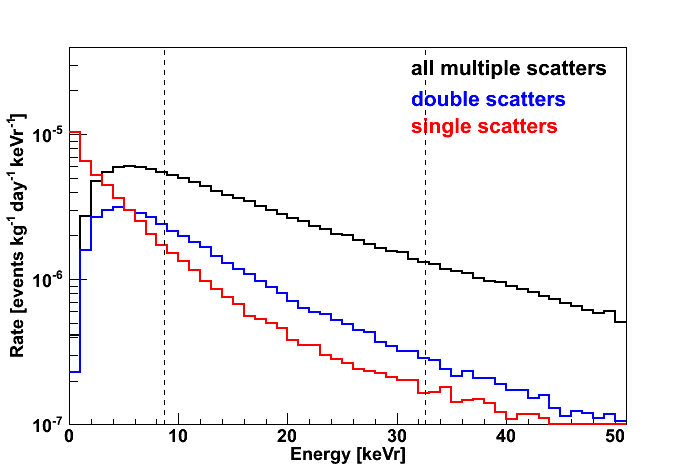
\includegraphics[width=0.475\linewidth]{plots/NRalphaN/Spectrum_alphan_SM_30kg.png}
\label{figAlphaNspectraSM_1}}
\subfigure[]{
%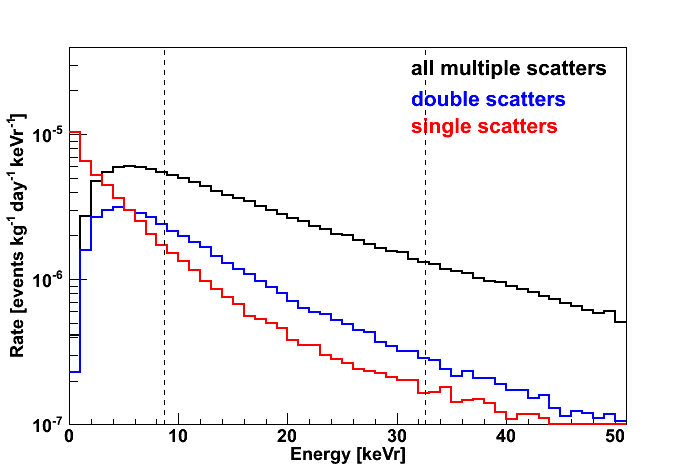
\includegraphics[width=0.475\linewidth]{plots/NRalphaN/Spectrum_alphan_SM_30kg.png}
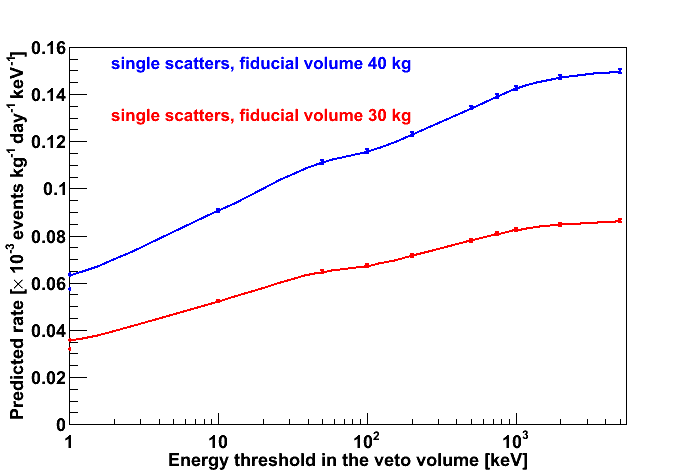
\includegraphics[width=0.475\linewidth]{plots/NRalphaN/VetoReduction_Neutrons_FV40andFV30.png}
\label{figAlphaNspectraSM_2}}
\caption[Energy spectra of nuclear recoils from neutrons produced in ($\alpha$,n) and spontaneous fission reactions, and efficiency of the veto coincidence cut as a function of the energy deposit in the veto volume]{(a) - energy spectra of nuclear recoils in 30~kg fiducial volume from neutrons produced in ($\alpha$,n) and spontaneous fission reactions. (b) - efficiency of the veto coincidence cut as a function of the energy deposit in the veto volume. The vertical dashed lines indicate the energy region used for analysis of the commissioning run in Fall 2009 (run07~\cite{xe100-run07}). Energy deposited in multiple scatter neutron interactions is in average higher than that in single scatter events. A veto cut with the volume averaged energy threshold of 100~keV$_{\mathrm{ee}}$ provides 20$-$30\% background reduction.}
\label{figAlphaNspectraSM}
\end{figure}

\begin{figure}[!b]
\centering
\subfigure[single scatter events]{
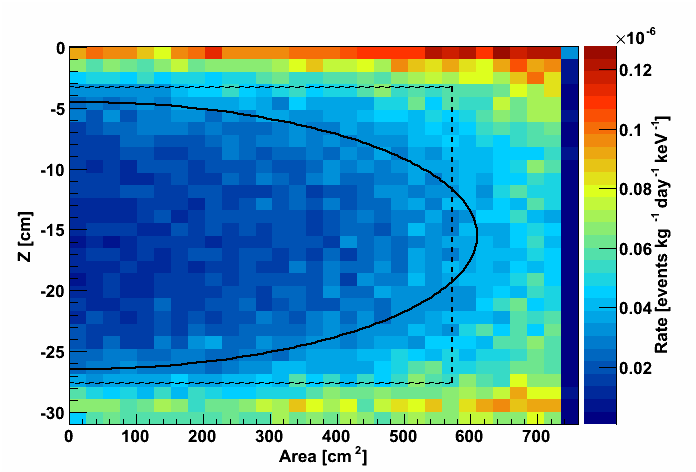
\includegraphics[width=0.475\linewidth]{plots/NRalphaN/sum_AZ.png}
\label{figAlphaNaz_1}}
%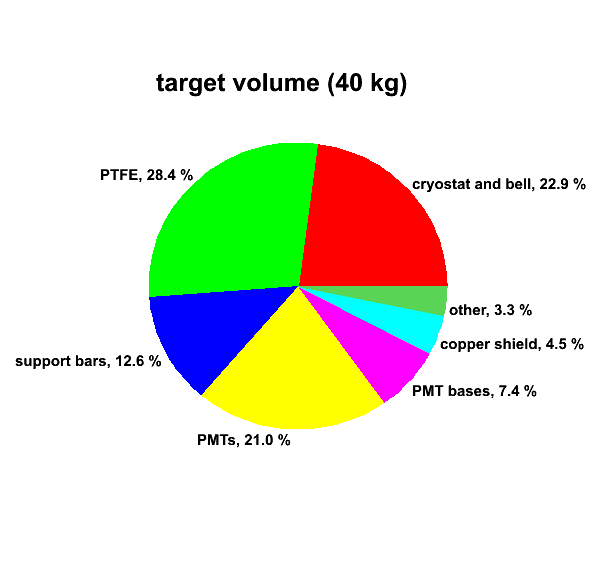
\includegraphics[width=0.475\linewidth]{plots/NRalphaN/AlphaN_Pie40kg.png}
\subfigure[multiple scatter events]{
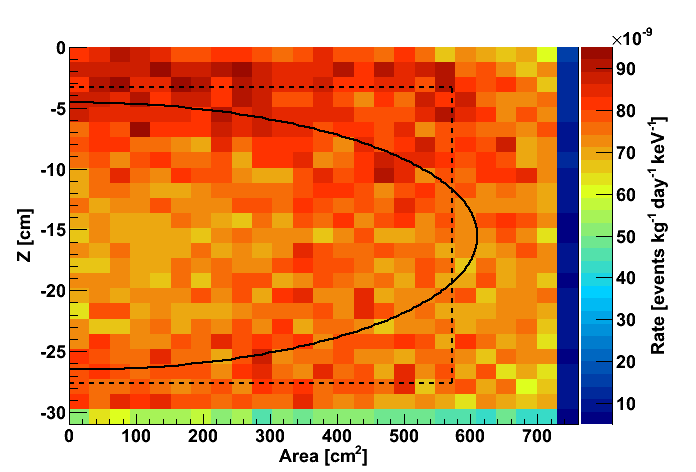
\includegraphics[width=0.475\linewidth]{plots/NRalphaN/AlphaN_AZ_MultipleScatters_xM_25bins.png}
\label{figAlphaNaz_2}}
\caption[Spatial distribution of nuclear recoils due to neutrons produced in ($\alpha$,n) and spontaneous fission reactions in the detector and shield components]{Spatial distribution of nuclear recoils due to neutrons produced in ($\alpha$,n) and spontaneous fission reactions in the detector and shield components: (a) - single scatter interactions, (b) - multiple scatter events. The position of multiples scatters has been defined by the position of the interaction with the highest energy deposition. Fiducialization is not as efficient for nuclear recoil background reduction as for the electronic recoil background due to longer attenuation length for neutrons in liquid xenon.}
\label{figAlphaNaz}
\end{figure}

The GEANT4.9.1.p02 version has been used for the neutron propagation in the detector and shield, together with the neutron data files with thermal cross sections G4NDL~3.13, which are based mostly on the ENDF/B-VI/B-VI databases~\cite{G4NDL}. For each material and neutron source, 1 million events have been simulated, resulting in a statistical uncertainty of $\sim$1\%.

In the analysis of the simulated data, only `pure' nuclear recoils have been selected. All events containing an electronic recoil component have been discarded. The single and multiple scatters are distinguished by taking into account the position resolution, introduced in Section~\ref{secPositionResolution}. The energy spectra of nuclear recoils produced in single and multiple scatter neutron interactions is shown for the 30~kg fiducial volume in Fig.~\ref{figAlphaNspectraSM_1}. In average, multiple scatter events have a higher energy deposition than single scatter interactions. By applying a veto coincidence cut with the measured volume averaged energy threshold of 100~keV$_{\mathrm{ee}}$, the background can be reduced by 20$-$30\% (Fig.~\ref{figAlphaNspectraSM_2}).

The spatial distribution of the nuclear recoils in the TPC is shown in Fig.~\ref{figAlphaNaz}. The position of multiple scatter events is shown as the position of the scatter with the highest energy deposition. Fiducialization is less efficient for the nuclear recoil background than for electronic recoils (see Section~\ref{secDetectorMaterials}) because of the longer mean free path of an MeV neutron, compared to a $\gamma$-ray of similar energy. The distribution of multiple scatter events is relatively uniform, resulting in a reduction of the single-to-multiple scatter ratio with a smaller fiducial volume, as shown in Table~\ref{tabAlphaNsmRatio}.

\begin{table}[!h]
\centering
\caption[Ratio of single and multiple scatter events in the energy region 8.7$-$32.6~keV$_{\mathrm{nr}}$ for different fiducial volumes]{Ratio of single and multiple scatter events in the energy region 8.7$-$32.6~keV$_{\mathrm{nr}}$ for different fiducial volumes.}
\label{tabAlphaNsmRatio}
\begin{tabular}{>\footnotesize{l} | >\footnotesize{c} | >\footnotesize{c} | >\footnotesize{c} | >\footnotesize{c}}
\hline
Volume 		     			& 62~kg 		& 48~kg  		& 40~kg 		& 30~kg \\
\hline
single/multiple	ratio			& 0.45 		& 0.32 		& 0.29		& 0.22 \\
single/double ratio			& 1.08 		& 0.85 		& 0.76		& 0.65 \\
\hline
\end{tabular}
\end{table}

\begin{table}[!h]
\centering
\caption[Predicted background rate of nuclear recoils in the energy range region of interest from neutrons produced in ($\alpha$,n) and spontaneous fission reactions, without veto cut]{Predicted background rate of nuclear recoils in the energy range 8.7$-$32.6~keV$_{\mathrm{nr}}$ from neutrons produced in ($\alpha$,n) and spontaneous fission reactions due to natural radioactivity in the detector an shield components, {\it without veto cut}. The statistical error of the GEANT4 simulation is $\sim$1\%. The systematic uncertainty of the neutron production rate calculation with SOURCES-4A is 17\%.}
\label{tabAlphaNratesPassiveVeto}
\begin{tabular}{>\footnotesize{l} | >\footnotesize{c} | >\footnotesize{c} | >\footnotesize{c} | >\footnotesize{c}}
\hline
				      		& \multicolumn{4}{>\footnotesize{c}}{Predicted background rate [year$^{-1}$]} \\
Volume 		     			& 62~kg 			& 48~kg  			& 40~kg 			& 30~kg \\
\hline
all events 					& 1.26$\pm$0.21 	& 0.94$\pm$0.16 	& 0.70$\pm$0.12 	& 0.50$\pm$0.09 \\
single scatter events			& 0.38$\pm$0.07	& 0.23$\pm$0.04 	& 0.15$\pm$0.03	& 0.09$\pm$0.02 \\
multiple scatter events		& 0.88$\pm$0.15 	& 0.71$\pm$0.12 	& 0.55$\pm$0.09	& 0.41$\pm$0.07 \\
double scatter events		& 0.35$\pm$0.06 	& 0.27$\pm$0.05 	& 0.20$\pm$0.03	& 0.13$\pm$0.02 \\
\hline
\end{tabular}
\end{table}

\begin{table}[!h]
\centering
\caption[Predicted background rate of nuclear recoils in the WIMP-search energy range from neutrons produced in ($\alpha$,n) and spontaneous fission reactions, with veto coincidence cut]{Predicted background rate of nuclear recoils in the energy range 8.7$-$32.6~keV$_{\mathrm{nr}}$ from neutrons produced in ($\alpha$,n) and spontaneous fission reactions due to natural radioactivity in the detector an shield components. A {\it veto coincidence cut} with a measured volume averaged energy threshold of 100~keV$_{\mathrm{ee}}$ provides a 20$-$30\% background reduction.}
\label{tabAlphaNratesActiveVeto}
\begin{tabular}{>\footnotesize{l} | >\footnotesize{c} | >\footnotesize{c} | >\footnotesize{c} | >\footnotesize{c}}
\hline
				      		& \multicolumn{4}{>\footnotesize{c}}{Predicted background rate [year$^{-1}$]} \\
Volume 		     			& 62~kg 			& 48~kg  			& 40~kg 			& 30~kg \\
\hline
all events 					& 0.91$\pm$0.16 	& 0.69$\pm$0.12 	& 0.51$\pm$0.09 	& 0.37$\pm$0.06 \\
single scatter events			& 0.29$\pm$0.05	& 0.18$\pm$0.03 	& 0.12$\pm$0.02	& 0.07$\pm$0.01 \\
multiple scatter events		& 0.62$\pm$0.11 	& 0.51$\pm$0.09 	& 0.39$\pm$0.07	& 0.30$\pm$0.05 \\
double scatter events		& 0.26$\pm$0.04 	& 0.20$\pm$0.03 	& 0.15$\pm$0.03	& 0.10$\pm$0.02 \\
\hline
\end{tabular}
\end{table}

\begin{figure}[!h]
\centering
\subfigure[62~kg]{
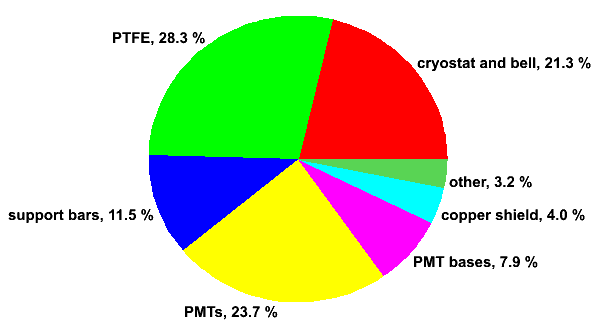
\includegraphics[width=0.475\linewidth]{plots/NRalphaN/AlphaN_Pie62kg_mod.png}
\label{figAlphaNpies_1}}
%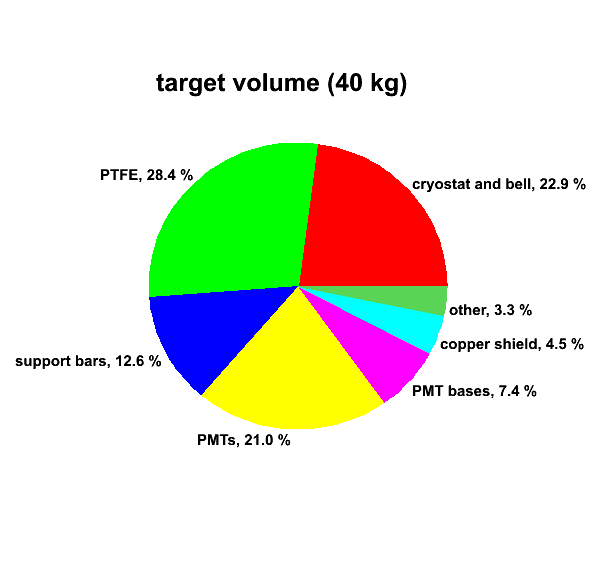
\includegraphics[width=0.475\linewidth]{plots/NRalphaN/AlphaN_Pie40kg.png}
\subfigure[30~kg]{
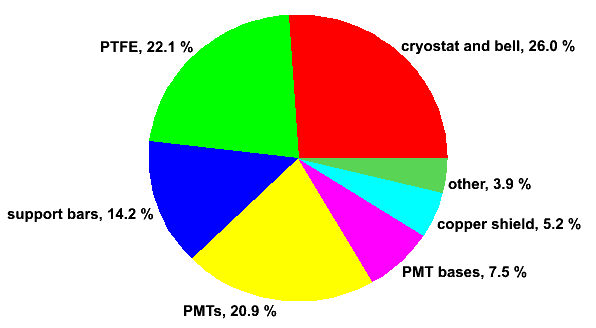
\includegraphics[width=0.475\linewidth]{plots/NRalphaN/AlphaN_Pie30kg_mod.png}
\label{figAlphaNpies_2}}
\caption[Contribution from different components to the total background from ($\alpha$,n) and spontaneous fission reactions]{Contribution from different components to the total single scatter background from ($\alpha$,n) and spontaneous fission reactions: (a) - in the entire liquid xenon target of 62~kg, (b) - in 30~kg fiducial volume. The dominant contributions are from the detector PTFE, PMTs, and the 316Ti SS of the cryostat, the supports bars, and the diving bell. The fractions almost do not change with fiducialization of the liquid xenon target.}
\label{figAlphaNpies}
\end{figure}

The predicted background rates are presented in Tables~\ref{tabAlphaNratesPassiveVeto} and \ref{tabAlphaNratesPassiveVeto}, without and with veto coincidence cut, respectively. The contribution of different detector and shield components to the total single scatter nuclear recoil background rate is shown in Fig.~\ref{figAlphaNpies}. The dominant part of the background comes from the detector PTFE, PMTs and the 316Ti SS of the cryostat and its support bars, and the diving bell. This has been expected due to the rather high neutron production rates in these components (see Section~\ref{secNRalphaN_SOURCES}), and their location close to liquid xenon target. The relative contribution almost does not change by applying fiducial volume and veto coincidence cuts.

%\begin{table}[!h]
%\centering
%\caption{Predicted background rate of nuclear recoils from neutrons produced in ($\alpha$,n) and spontaneous fission reactions due to natural radioactivity in the detector an shield components. The statistical error of the GEANT4 simulation is $\sim$1\%. The systematic uncertainty of the neutron production rate calculation with SOURCES-4A is 17\%. Veto coincidence cut with a measured volume averaged energy threshold of 100~keV$_{ee}$ has been used.}
%\label{tabAlphaNrates}
%\vspace{0.2cm}
%\begin{tabular}{>\footnotesize{l} | >\footnotesize{c} | >\footnotesize{c} | >\footnotesize{c} | >\footnotesize{c} | >\footnotesize{c} | >\footnotesize{c} | >\footnotesize{c} | >\footnotesize{c}}
%\hline
%				      		& \multicolumn{8}{>\footnotesize{c}}{Predicted background rate [year$^{-1}$]} \\
%Volume 		     			& \multicolumn{2}{>\footnotesize{c}}{62~kg} 	& \multicolumn{2}{>\footnotesize{c}}{48~kg}  	& \multicolumn{2}{>\footnotesize{c}}{40~kg} 	& \multicolumn{2}{>\footnotesize{c}}{30~kg} \\
%Veto cut 		     			& none 			& active	& none 	& active	& none 	& active	& none 	& active	 \\
%\hline
%all events 					& 1.26$\pm$0.21	& 	& 0.94$\pm$0.16	& 	& 0.70$\pm$0.12	& 	& 0.50$\pm$0.09	& \\
%single scatter events			& 0.38$\pm$0.07	&	& 0.23$\pm$0.04	& 	& 0.15$\pm$0.03	&	& 0.09$\pm$0.02	& \\
%multiple scatter events		& 0.88$\pm$0.15	& 	& 0.71$\pm$0.12	& 	& 0.55$\pm$0.09	&	& 0.41$\pm$0.07	& \\
%double scatter events		& 0.35$\pm$0.06	& 	& 0.27$\pm$0.05	& 	& 0.20$\pm$0.03	&	& 0.13$\pm$0.02	& \\
%\hline
%\end{tabular}
%\end{table}




